\documentclass{monochrome}

\begin{document}

\counterwithin{equation}{section}

\pagestyle{fancy}
\pagestyle{empty}

\begin{tikzpicture}[remember picture,overlay]
    \fill[cw1!90]
    (current page.north west) rectangle (current page.south east);
    \coordinate (start) at ($(current page.east)!0.5!(current page.north east)+(1,-1)$);
    \coordinate (end) at (current page.north west);
    \foreach \i in {0,0.01,...,1}
    {
        \coordinate (point) at ($(start)!\i!(end)$);
        \draw[cw0]
        ($(point)+(310*\i:6)$)--
        ($(point)+(310*\i+120:6)$)--
        ($(point)+(310*\i+240:6)$)--
        ($(point)+(310*\i:6)$);
    }
    \coordinate (start) at (current page.south west);
    \coordinate (end)   at (current page.east);
    \foreach \i in {0,0.02,...,1}
    {
        \coordinate (point) at ($(start)!\i!(end)$);
        \draw[cw0]
        ($(point)+(310*\i:10)$)--
        ($(point)+(310*\i+120:10)$)--
        ($(point)+(310*\i+240:10)$)--
        ($(point)+(310*\i:10)$);
    }
    \shade[bottom color=cw2, top color=cw2!70, opacity=0.65] ([xshift=.5\outermarginwidth]current page.north west) rectangle (current page.south east);
    \shade[left color=cw0!40, right color=cw0!50, opacity=0.5] ([xshift=\outermarginwidth, yshift=2\outermarginwidth]current page.west) rectangle (current page.south east);
    \fill[cw0]([yshift=2\outermarginwidth]current page.west) rectangle ([xshift=\outermarginwidth, yshift=-.2\outermarginwidth]current page.west);
    \foreach \lx/\rx/\ry/\bc/\tc in {
            1/1.5/1.75/70/80,1.5/2/1.6/65/75,2/2.5/1.3/60/70,2.5/3/1/55/65,3/3.5/.7/50/60,3.5/4/1.2/60/70,4/4.5/1.9/75/85,4.5/5/1.1/55/65,5/5.5/1.2/60/70,6/6.5/1.6/65/75,6.5/7/1.3/60/70,7/7.5/1.87/70/80,7.5/8/1/55/65,8/8.5/.9/50/60,8.5/9/1.8/70/80,9/9.5/1.6/65/75,9.5/10/1.4/60/70,10/10.5/1/55/65,10.5/11/.7/50/60,11/11.5/1.3/55/65,11.5/12/1/70/80,12/12.5/1.3/65/75,12.5/13/1.6/60/70,13/13.5/1.75/55/65,13.5/14/1.6/65/75,14/14.5/1.3/60/70
    }{
        \shade[bottom color=cw0!\bc,top color=cw3!\tc,opacity=.3]
        ([xshift=\lx\outermarginwidth]current page.north west) rectangle ([xshift=\rx\outermarginwidth,yshift=-\ry\covershift]current page.north west);
    }
    %%%%%% LETRAS %%%%%
    \node[anchor=south,right] at ([xshift=-5.55\outermarginwidth, yshift=-.465\paperheight]current page.north) {\selectfont           \color{cw0}\cabin\bfseries\fontsize{74}{74}\selectfont MATEMÁTICAS};
    \node[anchor=south,right] at ([xshift=-5.65\outermarginwidth, yshift=-.57\paperheight]current page.north) {\selectfont           \color{cw0}\cabin\bfseries\fontsize{74}{74}\selectfont DISCRETAS};
    \node[anchor=west, font=\cabin\fontsize{23}{23}\selectfont, text=white] at ([xshift=1.5\outermarginwidth, yshift=-1.25\covershift]current page.west) {Una introducción con aplicaciones};
    \node[anchor=west, font=\cabin\LARGE, text=black] at ([xshift=-2.25\outermarginwidth, yshift=-2.3\covershift]current page.center) {Antonio M. Mendoza ~$\bullet$~ Ramón V. Palomares};
\end{tikzpicture}

\newpage
\,

\newpage

\symmetricalPage%

\begin{tikzpicture}[remember picture,overlay]%
      \coordinate (A) at ($(current page.north)!.4!(current page.north east)$);
      \coordinate (B) at (current page.east);
      \coordinate (C) at (current page.north east);

      \filldraw[cw0!50] (A) -- (B) -- (C) -- cycle;
      \filldraw[cw0] ($(current page.north)!.4!(current page.north east)+(0.5,0)$) -- ($(current page.east)+(0,0.25)$) -- (C) -- cycle;
\end{tikzpicture}


\vspace{2cm}
\begin{center}
\scalebox{5.5}{\fontencoding{T1}\fontfamily{pag}\selectfont\textbf{\color{cw0}MATEMÁTICAS}}\\[10mm]
\scalebox{5.5}{\fontencoding{T1}\fontfamily{pag}\selectfont\textbf{\color{cw2}DISCRETAS}}\\[2cm]

\begin{tabular}{c} \selectfont\cabin\scalebox{2}{Rubén Ramón} \\[2mm] \selectfont\cabin\scalebox{2}{Vargas Palomares} \end{tabular} \hspace{2.5cm} \begin{tabular}{c} \selectfont\cabin\scalebox{2}{Marco Antonio} \\[2mm] \selectfont\cabin\scalebox{2}{Molina Mendoza} \end{tabular}\\[26mm]

\begin{center}
    \begin{tikzpicture}
        \node at (current page.center) {
\includegraphics[width=0.3\textwidth]{Images/Portada/POLITECNICO.pdf}}; % Logo de institución
    \end{tikzpicture}
\end{center}
\fontencoding{T1}\fontfamily{pag}\selectfont Instituto Politécnico Nacional

\vfill
~%México, 2024
\end{center}

\newpage
\,

\newpage

~\vfill\hfill\begin{minipage}[l]{0.6\textwidth}
     \selectfont\cabin\itshape Quiero expresar mi agradecimiento al Dr. Rubén Ramón Vargas Palomares, quien aparte de haber sido mi profesor, me permitió recopilar el presente trabajo.
\end{minipage}

\restoregeometry%

\newpage
\,

\renewcommand{\contentsname}{CONTENIDO}
\hypersetup{hidelinks}
\TOCPage%
\tableofcontents
\label{toc-contents}
\restoregeometry

\pagestyle{fancy}

%\input{tex/prefacio}

%\input{tex/bibliografia}

\part{FUNDAMENTOS DE LA MATEMÁTICA DISCRETA}

\chapter{FUNDAMENTOS DE LA LÓGICA}
\printchaptertableofcontents

En este capítulo, examinaremos con detenimiento qué constituye un argumento válido y una demostración más convencional. Cuando un matemático quiere demostrar un resultado, debe utilizar un sistema lógico. Lo mismo ocurre cuando un científico de la computación desarrolla algoritmos para un programa o un conjunto de programas. La lógica matemática se aplica para determinar si una afirmación se deduce de, o es una consecuencia lógica de, otras afirmaciones previas.

Algunas de las reglas que guían este proceso se describen en este capítulo. Utilizaremos estas reglas en las pruebas que aparecerán en el texto y en los ejercicios de los capítulos siguientes. Sin embargo, nunca llegaremos a un punto en el que podamos aplicar estas reglas de manera automática. Limitarse a aplicar fórmulas o reglas no nos llevará muy lejos, ya sea en la demostración de teoremas o en la resolución de problemas de conteo.

\section{Conectivos y tablas de verdad}

En el desarrollo de cualquier teoría matemática, se hacen afirmaciones en forma de oraciones. Estas afirmaciones verbales o escritas, llamadas enunciados (o proposiciones), son oraciones declarativas que son verdaderas o falsas, pero no ambas a la vez. Por ejemplo, los siguientes son enunciados, y utilizamos letras minúsculas del alfabeto (como $p$, $q$ y $r$) para representar estos enunciados.
\begin{align*}
    p: & \quad \text{El Álgebra es un curso obligatorio para los estudiantes de primer año.} \\
    q: & \quad \text{Diana Bravo escribió \emph{Lo que el viento se llevó}.} \\
    r: & \quad 2 + 3 = 5.
\end{align*}\newpage\noindent
Por otro lado, no consideramos oraciones como la exclamación
\begin{nscenter}
    “¡Qué hermosa noche!”
\end{nscenter}
o la orden
\begin{nscenter}
    “Levántate y haz tus ejercicios”
\end{nscenter}
como enunciados, ya que no poseen valores de verdad (verdadero o falso).

Los enunciados anteriores, representados por las letras $p$, $q$, y $r$, se consideran enunciados primitivos, ya que realmente no hay manera de descomponerlos en algo más simple. A partir de estos enunciados, se pueden obtener nuevos enunciados de dos maneras.
\begin{enumerate}
    \item Para transformar una afirmación dada $p$ en su negación $\neg p$, simplemente le agregamos “no” a la afirmación original. Por ejemplo, si
    $$p: \quad \text{Diana Bravo escribió \emph{Lo que el viento se llevó}}$$
    entonces $\neg p$ sería
    $$\neg p: \quad \text{Diana Bravo no escribió \emph{Lo que el viento se llevó}}$$
    Es importante destacar que la negación de una afirmación primitiva no se considera una afirmación primitiva en sí misma.
    \item Combinando dos o más enunciados en una proposición compuesta, utilizando los siguientes conectores lógicos.
    \begin{enumerate}
        \item Conjunción: La conjunción de las afirmaciones $p$ y $q$ se denota por $p \land q$, que se lee “$p$ y $q$”. En nuestro ejemplo, la afirmación compuesta $p \land q$ se lee “El Álgebra es un curso obligatorio para los estudiantes de primer año, y Diana Bravo escribió \emph{Lo que el viento se llevó}”.
        \item Disyunción: La expresión $p \lor q$ denota la disyunción de las afirmaciones $p$ y $q$, y se lee “$p$ o $q$”. Así, “El Álgebra es un curso obligatorio para los estudiantes de primer año, o y Diana Bravo escribió \emph{Lo que el viento se llevó}” es la traducción verbal de $p \lor q$, cuando $p$ y $q$ son como se describió anteriormente. Aquí usamos la palabra “o” en el sentido inclusivo. En consecuencia, $p \lor q$ es verdadero si una de las afirmaciones $p$ o $q$ es verdadera, o si ambas lo son. En español, a veces se escribe “y/o” para señalar esto. La “o” exclusiva se denota por $p \veebar q$. La afirmación compuesta $p \veebar q$ es verdadera si una de las afirmaciones $p$ o $q$ es verdadera, pero no ambas. Una forma de expresar $p \veebar q$ en este ejemplo es “El Álgebra es un curso obligatorio para los estudiantes de primer año, o y Diana Bravo escribió \emph{Lo que el viento se llevó}, pero no ambas cosas”.
        \item Implicación: Decimos que “$p$ implica $q$” y escribimos $p \rightarrow q$ para designar la afirmación, lo que es la implicación de $q$ por $p$. Alternativamente, también podemos decir:
        \begin{tasks}[label=\roman*)](2)
            \task “Si $p$, entonces $q$”.
            \task “$p$ es suficiente para $q$”.
            \task*(2) “$p$ es una condición suficiente para $q$”.
            \task*(2) “$q$ es una condición necesaria para $p$”.
            \task “$q$ es necesario para $p$”.
            \task “$p$ solo si $q$”.
        \end{tasks}
        Una traducción verbal de $p \rightarrow q$ en nuestro ejemplo sería: “Si el Álgebra es un curso obligatorio para los estudiantes de primer año, entonces Diana Bravo escribió \emph{Lo que el viento se llevó}”. La afirmación $p$ se denomina la hipótesis de la implicación; $q$ se denomina la conclusión. Cuando se combinan afirmaciones de esta manera, no es necesario que exista una relación causal entre ellas para que la implicación sea verdadera.\newpage
        \item Bicondicional o equivalencia: Finalmente, el bicondicional de dos afirmaciones $p$ y $q$ se denota por $p \leftrightarrow q$, lo cual se lee como “$p$ si y solo si $q$”, o “$p$ es necesario y suficiente para $q$”. En nuestro ejemplo, “El Álgebra es un curso obligatorio para los estudiantes de primer año si y solo si Diana Bravo escribió \emph{Lo que el viento se llevó}” transmite el significado de $p \leftrightarrow q$. A veces, se abrevia como "$p$ si y solo si $q$" o simplemente “$p$ sii $q$”.
    \end{enumerate}
\end{enumerate}
La siguiente tabla resume lo dicho anteriormente:
\begin{table*}[h!]
    \centering
    \begin{NiceTabular}{cccc}[hvlines-except-borders, cell-space-limits=4pt, rules={color=white,width=1pt}]
        \CodeBefore
        \rowcolor{cw0!80}{1}
        \rowcolors{2}{cw2!70!white}{cw1!30!white}
        \Body
        \RowStyle[color=white]{}
        \RowStyle{\bfseries}Tipo de enunciado & Símbolo & Descripción & Ejemplo \\
        Enunciados primitivos & $p$, $q$, $r$ & \makecell{Enunciados básicos que no pueden \\ descomponerse en algo más simple} & \makecell{“Diana Bravo escribió \\ \emph{Lo que el viento se llevó}”} \\
        Negación & $\neg p$ & \makecell{Se niega un enunciado añadiendo \\ “no” a la afirmación original. La \\ negación de una afirmación primitiva \\ no es una afirmación primitiva} & \makecell{“Diana Bravo no escribió \\ \emph{Lo que el viento se llevó}”} \\
        Conjunción & $p \land q$ & \makecell{La combinación de dos enunciados con \\ “y”. El compuesto es verdadero solo \\ si ambos enunciados son verdaderos} & \makecell{“El Álgebra es obligatorio, \\ y Diana Bravo escribió \\ \emph{Lo que el viento se llevó}”} \\
        \makecell{Disyunción\\ (disyunción inclusiva)} & $p \lor q$ & \makecell{La combinación de dos enunciados con \\ “o”. El compuesto es verdadero si al \\ menos uno de los enunciados es verdadero} & \makecell{“El Álgebra es obligatorio, \\ o Diana Bravo escribió \\ \emph{Lo que el viento se llevó}”} \\
        Disyunción exclusiva & $p \veebar q$ & \makecell{Es verdadero si exactamente uno de los \\ enunciados es verdadero, pero no ambos} & \makecell{“El Álgebra es obligatorio, \\ o Diana Bravo escribió \\ \emph{Lo que el viento se llevó}, \\ pero no ambas cosas”} \\
        Implicación & $p \rightarrow q$ & \makecell{Indica que si $p$ es verdadero, entonces \\ $q$ también lo es. No requiere una \\ relación causal entre $p$ y $q$} & \makecell{“Si el Álgebra es obligatorio, \\ entonces Diana Bravo escribió \\ \emph{Lo que el viento se llevó}”} \\
        Bicondicional & $p \leftrightarrow q$ & \makecell{Indica que $p$ es verdadero si y solo si \\ $q$ es verdadero. Se considera tanto \\ necesario como suficiente para \\ que $p$ implique $q$ y viceversa} & \makecell{“El Álgebra es obligatorio si y \\ solo si Diana Bravo escribió \\ \emph{Lo que el viento se llevó}”}
    \end{NiceTabular}
    \caption{}
\end{table*}

A lo largo de nuestra discusión sobre lógica, debemos darnos cuenta de que una oración como
\begin{nscenter}
    “El número $x$ es un entero”
\end{nscenter}
no es una proposición porque su valor de verdad (verdadero o falso) no puede determinarse hasta que se asigne un valor numérico a $x$. Si se le asigna a $x$ el valor de 7, el resultado sería una proposición verdadera. Sin embargo, si se le asigna a $x$ un valor como $3.27$ o $\pi$, la proposición resultante sería falsa.

En la discusión anterior, mencionamos en qué circunstancias las proposiciones compuestas $p \lor q$ y $p \veebar q$ se consideran verdaderas, basándonos en la verdad de sus componentes $p$ y $q$. Esta idea, de que la verdad o falsedad de una proposición compuesta depende únicamente de los valores de verdad de sus componentes, merece una investigación más profunda. Las tablas \ref{tab:tabladeverdad1} y \ref{tab:tabladeverdad2} resumen la verdad y falsedad de la negación y de los diferentes tipos de proposiciones compuestas en función de los valores de verdad de sus componentes. Al construir estas tablas de verdad, usamos “$0$” para falso y “$1$” para verdadero.\infoBulle{Las cuatro asignaciones posibles de verdad para $p$ y $q$ se pueden listar en cualquier orden. Sin embargo, para trabajos posteriores, el orden particular presentado aquí resultará útil.}
\begin{nscenter}
    \hspace{-0.5cm}\begin{minipage}[c]{0.15\textwidth}\vspace{1.18cm}
        \begin{NiceTabular}{cc}[hvlines-except-borders, cell-space-limits=4pt, rules={color=white,width=1pt}]
        \CodeBefore
        \rowcolor{cw0!80}{1}
        \rowcolors{2}{cw2!70!white}{cw1!30!white}
        \Body
        \RowStyle[color=white]{}
            $p$ & $\neg p$ \\
            0 & 1 \\
            1 & 0 \\ 
        \end{NiceTabular}
        \captionof{table}{}\label{tab:tabladeverdad1}
    \end{minipage}
\hspace{0.5cm}
    \begin{minipage}[c]{0.6\textwidth}
        \begin{NiceTabular}{ccccccc}[hvlines-except-borders, cell-space-limits=4pt, rules={color=white,width=1pt}]
        \CodeBefore
        \rowcolor{cw0!80}{1}
        \rowcolors{2}{cw2!70!white}{cw1!30!white}
        \Body
        \RowStyle[color=white]{}
            $p$ & $q$ & $p \land q$ & $p \lor q$ & $p \veebar q$ & $p \rightarrow q$ & $p \leftrightarrow q$ \\
            0 & 0 & 0 & 0 & 0 & 1 & 1 \\
            0 & 1 & 0 & 1 & 1 & 1 & 0 \\ 
            1 & 0 & 0 & 1 & 1 & 0 & 0 \\
            1 & 1 & 1 & 1 & 0 & 1 & 1 \\ 
        \end{NiceTabular}
        \captionof{table}{}\label{tab:tabladeverdad2}
    \end{minipage}
\end{nscenter}

Podemos observar que las columnas de valores de verdad para $p$ y $\neg p$ son opuestas entre sí. La afirmación $p \land q$ es verdadera solo cuando $p$ y $q$ son verdaderas, mientras que $p \lor q$ es falsa solo cuando ambas afirmaciones componentes, $p$ y $q$, son falsas. Como se mencionó anteriormente, $p \veebar q$ es verdadera cuando exactamente una de $p$ o $q$ es verdadera. En cuanto a la implicación $p \rightarrow q$, el resultado es verdadero en todos los casos, excepto cuando $p$ es verdadero y $q$ es falso. No queremos que una afirmación verdadera nos lleve a creer algo que es falso. Sin embargo, consideramos verdadera una afirmación como “Si $2 + 3 = 6$, entonces $2 + 4 = 7$", a pesar de que ambas afirmaciones “$2 + 3 = 6$” y “$2 + 4 = 7$” son falsas. Finalmente, el bicondicional $p \leftrightarrow q$ es verdadero cuando las afirmaciones $p$ y $q$ tienen el mismo valor de verdad y es falso en caso contrario.

Ahora que hemos sido introducidos a ciertos conceptos, analicemos un poco más algunas de estas ideas iniciales sobre los conectores lógicos.
\begin{examplebox}{}{}
    Sean $s$, $t$ y $u$ las siguientes proposiciones primitivas:
    \begin{align*}
        s: & \quad \text{Phyllis sale a dar un paseo.} \\
        t: & \quad \text{La luna está brillando.} \\
        u: & \quad \text{Está nevando.}
    \end{align*}
    Las siguientes oraciones en español ofrecen posibles traducciones para los enunciados compuestos (simbólicos) dados.
    \begin{enumerate}[label=\alph*), topsep=6pt, itemsep=0pt]
        \item $(t \land \neg u) \rightarrow s$: Si la luna está brillando y no está nevando, entonces Phyllis sale a dar un paseo.
        \item $t \rightarrow (\neg u \rightarrow s)$: Si la luna está brillando, entonces si no está nevando, Phyllis sale a dar un paseo. De esta forma, la proposición compuesta $\neg u \rightarrow s$ se entiende como $(\neg u) \rightarrow s$, en lugar de $\neg (u \rightarrow s)$.
        \item $\neg(s \leftrightarrow (u \lor t))$: No ocurre que Phyllis salga a dsr un paseo si y solo si está nevando o la luna está brillando.
    \end{enumerate}
    Ahora trabajaremos en orden inverso y examinaremos la notación lógica (o simbólica) para tres oraciones dadas:
    \begin{enumerate}[resume, label=\alph*), topsep=6pt, itemsep=0pt]
        \item “Phyllis saldrá a dar un paseo si y solo si la luna está brillando”. Aquí, las palabras “si y solo si” indican que estamos tratando con un bicondicional. En forma simbólica, esto se expresa como $s \leftrightarrow t$.
        \item “Si está nevando y la luna no está brillando, entonces Phyllis no saldrá a dar un paseo”. Esta proposición compuesta es una implicación donde la hipótesis también es una afirmación compuesta. Se puede expresar esta afirmación en forma simbólica como $(u \land \neg t) \rightarrow \neg s$.
        \item “Está nevando, pero Phyllis aún saldrá a dar un paseo”. Aquí encontramos un nuevo conector: “pero”. En nuestro estudio de lógica, seguiremos la convención de que los conectores “pero” e “y” tienen el mismo significado. Por lo tanto, esta oración se puede representar simbólicamente como $u \land s$.
    \end{enumerate}
\end{examplebox}

\newpage

\begin{examplebox}{}{}
    En ciencias de la computación, las estructuras de decisión \textbf{if-then} e \textbf{if-then-else} surgen (en varios formatos) en lenguajes de programación de alto nivel como Java y C. La hipótesis $p$ suele ser una expresión relacional, como $x > 2$. Esta expresión se convierte en una declaración lógica que tiene un valor de verdad de 0 o 1, dependiendo del valor de la variable $x$ en ese punto del programa. La conclusión $q$ suele ser una “instrucción ejecutable” (por lo tanto, $q$ no es una de las declaraciones lógicas que hemos estado analizando). Cuando se trata de “si $p$ entonces $q$”, en este contexto, la computadora ejecuta $q$ solo si $p$ es verdadero. Si $p$ es falso, la computadora pasa a la siguiente instrucción en la secuencia del programa. Para la estructura de decisión “si $p$ entonces $q$ de lo contrario $r$”, $q$ se ejecuta cuando $p$ es verdadero y $r$ se ejecuta cuando $p$ es falso.

    \hspace{15pt}La instrucción de selección \mintinline{C}{if} realiza una acción indicada, solo cuando la condición es verdadera; de lo contrario, se ignora dicha acción. La instrucción de selección \mintinline{C}{if...else} permite al programador especificar que se realizarán acciones diferentes cuando la condición sea verdadera y cuando la condición sea falsa. Por ejemplo, la instrucción en pseudocódigo
    \begin{minted}[escapeinside=]{C}
    if calificación del estudiante es mayor o igual que 60
        Imprime "Aprobado"
    else
        Imprime "Reprobado"
    \end{minted}
    imprime \mintinline{tex}{Aprobado} si la calificación del estudiante es mayor o igual que 60, e imprime \mintinline{tex}{Reprobado} si la calificación del estudiante es menor que 60. La instrucción \mintinline{C}{if...else} del pseudocódigo anterior se puede escribir en C como:
    \begin{minted}[escapeinside=]{C}
    if (calificación >= 60)
        printf("Aprobado\n");
    else
        printf("Reprobado\n");
    \end{minted}
\end{examplebox}

\begin{examplebox}{}{}
    Examinemos la tabla de verdad para la proposición compuesta: “Diana Bravo escribió \emph{Lo que el viento se llevó}, y si $2 + 3 \neq 5$, entonces el Álgebra es un curso obligatorio para los estudiantes de primer año”, que en notación simbólica se representa como $q \land (\neg r \rightarrow p)$, donde $p$, $q$, y $r$ son los enunciados primitivos mencionados al inicio de esta sección. La última columna de la tabla \ref{tab:tabladeverdad3} muestra los valores de verdad de esta expresión. Estos valores se obtienen considerando que la conjunción de dos enunciados es verdadera solo si ambos son verdaderos, los cuales se obtienen descomponiendo la proposición en partes más simples y aplicando los resultados de las tablas \ref{tab:tabladeverdad1} y \ref{tab:tabladeverdad2}.
    \begin{nscenter}
        \begin{NiceTabular}{cccccc}[hvlines-except-borders, cell-space-limits=4pt, rules={color=white,width=1pt}]
        \CodeBefore
        \rowcolor{cw0!80}{1}
        \rowcolors{2}{cw2!70!white}{cw1!30!white}
        \Body
        \RowStyle[color=white]{}
            $p$ & $q$ & $r$ & $\neg r$ & $r \rightarrow p$ & $q \land \left( \neg r \rightarrow p \right)$ \\ 
            0 & 0 & 0 & 1 & 0 & 0 \\
            0 & 0 & 1 & 0 & 1 & 0 \\ 
            0 & 1 & 0 & 1 & 0 & 0 \\
            0 & 1 & 1 & 0 & 1 & 1 \\
            1 & 0 & 0 & 1 & 1 & 0 \\
            1 & 0 & 1 & 0 & 1 & 0 \\
            1 & 1 & 0 & 1 & 1 & 1 \\
            1 & 1 & 1 & 0 & 1 & 1
        \end{NiceTabular}
        \captionof{table}{}\label{tab:tabladeverdad3}
    \end{nscenter}
\end{examplebox}

\newpage

\begin{examplebox}{}{}
    En la tabla \ref{tab:tabladeverdad4}, desarrollamos las tablas de verdad para las proposiciones compuestas $p \lor (q \land r)$ y $(p \lor q) \land r$.
    \begin{nscenter}
        \begin{NiceTabular}{ccccccc}[hvlines-except-borders, cell-space-limits=4pt, rules={color=white,width=1pt}]
        \CodeBefore
        \rowcolor{cw0!80}{1}
        \rowcolors{2}{cw2!70!white}{cw1!30!white}
        \Body
        \RowStyle[color=white]{}
            $p$ & $q$ & $r$ & $q \land r$ & $p \lor (q \land r)$ & $p \lor q$ & $(p \lor q) \land r$ \\
            0 & 0 & 0 & 0 & 0 & 0 & 0 \\
            0 & 0 & 1 & 0 & 0 & 0 & 0 \\
            0 & 1 & 0 & 0 & 0 & 1 & 0 \\
            0 & 1 & 1 & 1 & 1 & 1 & 1 \\
            1 & 0 & 0 & 0 & 1 & 1 & 0 \\
            1 & 0 & 1 & 0 & 1 & 1 & 1 \\
            1 & 1 & 0 & 0 & 1 & 1 & 0 \\
            1 & 1 & 1 & 1 & 1 & 1 & 1
        \end{NiceTabular}
        \captionof{table}{}\label{tab:tabladeverdad4}
    \end{nscenter}
    Debido a que los valores de verdad en las columnas 5 y 7 difieren (en las filas 5 y 7), debemos evitar escribir una proposición compuesta como $p \lor q \land r$ sin paréntesis para indicar cuál de los conectores lógicos $\lor$ y $\land$ se debe aplicar primero. Sin los paréntesis, no sabemos si estamos tratando con $p \lor (q \land r)$ o $(p \lor q) \land r$.
\end{examplebox}

\begin{examplebox}{}{}
    Los resultados en las columnas 4 y 7 de la tabla \ref{tab:tabladeverdad5} revelan que la afirmación $p \rightarrow (p \lor q)$ es verdadera y que la afirmación $p \land (\neg p \land q)$ es falsa para todas las asignaciones de valores de verdad a las afirmaciones componentes $p$ y $q$.
    \begin{nscenter}
        \begin{NiceTabular}{ccccccc}[hvlines-except-borders, cell-space-limits=4pt, rules={color=white,width=1pt}]
        \CodeBefore
        \rowcolor{cw0!80}{1}
        \rowcolors{2}{cw2!70!white}{cw1!30!white}
        \Body
        \RowStyle[color=white]{}
            $p$ & $q$ & $p \lor q$ & $p \rightarrow (p \lor q)$ & $\neg p$ & $\neg p \land q$ & $p \land (\neg p \land q)$ \\
            0 & 0 & 0 & 1 & 1 & 0 & 0 \\
            0 & 1 & 1 & 1 & 1 & 1 & 0 \\
            1 & 0 & 1 & 1 & 0 & 0 & 0 \\
            1 & 1 & 1 & 1 & 1 & 0 & 0
        \end{NiceTabular}
        \captionof{table}{}\label{tab:tabladeverdad5}
    \end{nscenter}
\end{examplebox}

\begin{definicion}{}{}
    Una proposición compuesta se llama una \emph{tautología} si es verdadera bajo cualquier asignación de valores de verdad a sus componentes. Si una proposición compuesta es falsa en todas estas asignaciones, entonces se le llama \emph{contradicción}.
\end{definicion}

A lo largo de este capítulo utilizaremos el símbolo $T_0$ para denotar cualquier tautología y el símbolo $F_0$ para denotar cualquier contradicción.

Podemos usar las ideas de tautología e implicación para describir lo que entendemos por un argumento válido. Esto será de gran interés para nosotros en la sección 1.3 y nos ayudará a desarrollar las habilidades necesarias para demostrar teoremas matemáticos. En general, un argumento comienza con una lista de enunciados llamados premisas y un enunciado llamado la conclusión del argumento. Si todas las premisas $p_1, p_2, p_3, \dots, p_n$ son verdaderas, entonces la conclusión $q$ también es verdadera. Una forma de hacerlo es examinando la implicación
$$(p_1 \land p_2 \land p_3 \land \cdots \land p_n) \rightarrow p$$
donde la hipótesis es la conjunción de las $n$ premisas. Si alguna de las premisas $p_1, p_2, p_3, \dots, p_n$ es falsa, entonces, sin importar cuál sea el valor de verdad de $q$, la implicación $(p_1 \land p_2 \land p_3 \land \cdots \land p_n) \rightarrow q$ será verdadera. Por lo tanto, si partimos de las premisas $p_1, p_2, p_3, \dots, p_n$, y cada una tiene un valor de verdad 1, y encontramos que bajo estas condiciones $q$ también tiene un valor de 1, entonces la implicación
$$(p_1 \land p_2 \land p_3 \land \cdots \land p_n) \rightarrow p$$
es una tautología y tenemos un argumento válido.

\section{Equivalencia lógica: Las leyes de la lógica}

En todas las áreas de las matemáticas, es fundamental reconocer cuándo las entidades que estamos estudiando son iguales o esencialmente equivalentes. Por ejemplo, en aritmética y álgebra sabemos que dos números reales no nulos son iguales cuando tienen la misma magnitud y el mismo signo algebraico. Así, para dos números reales no nulos $x$ e $y$, tenemos que $x = y$ si $|x| = |y|$ y $xy > 0$, y viceversa (es decir, si $x = y$, entonces $|x| = |y|$ y $xy > 0$). En geometría, cuando trabajamos con triángulos, surge la noción de congruencia. Aquí, el triángulo $ABC$ y el triángulo $DEF$ son congruentes si, por ejemplo, tienen lados correspondientes iguales, es decir, la longitud del lado $AB$ es igual a la longitud del lado $DE$, la longitud del lado $BC$ es igual a la longitud del lado $EF$, y la longitud del lado $CA$ es igual a la longitud del lado $FD$.

El estudio de la lógica a menudo se conoce como el \emph{álgebra de proposiciones} (en contraposición al álgebra de los números reales). En esta álgebra, utilizaremos las tablas de verdad de las proposiciones o enunciados para desarrollar una idea de cuándo dos de estas entidades son esencialmente iguales. Comencemos con el siguiente ejemplo

\begin{examplebox}{}{}
    Para los enunciados primitivos $p$ y $q$, la tabla \ref{tab:tabladeverdad6} muestra las tablas de verdad de las proposiciones compuestas $\neg p \lor q$ y $p \rightarrow q$. Aquí podemos observar que las tablas de verdad correspondientes para ambos enunciados, $\neg p \lor q$ y $p \rightarrow q$, son exactamente iguales.
    \begin{nscenter}
        \begin{NiceTabular}{ccccc}[hvlines-except-borders, cell-space-limits=4pt, rules={color=white,width=1pt}]
        \CodeBefore
        \rowcolor{cw0!80}{1}
        \rowcolors{2}{cw2!70!white}{cw1!30!white}
        \Body
        \RowStyle[color=white]{}
            $p$ & $q$ & $\neg p$ & $\neg p \lor q$ & $p \rightarrow q$ \\
            0 & 0 & 1 & 1 & 1 \\
            0 & 1 & 1 & 1 & 1 \\
            1 & 0 & 0 & 0 & 0 \\
            1 & 1 & 0 & 1 & 1
        \end{NiceTabular}
        \captionof{table}{}\label{tab:tabladeverdad6}
    \end{nscenter}
\end{examplebox}

El anterior ejemplo nos lleva a la siguiente definición

\begin{definicion}{}{}
    Dos enunciados $s_1$ y $s_2$ se dicen lógicamente equivalentes, y se escribe $s_1 \Leftrightarrow s_2$, cuando el enunciado $s_1$ es verdadero (o falso) si y solo si el enunciado $s_2$ es verdadero (o falso).
\end{definicion}

En otras palabras, $s_1$ y $s_2$ son lógicamente equivalentes cuando sus tablas de verdad tienen los mismos valores.

Como resultado de esta definición, podemos ver que es posible expresar el conector de implicación (entre enunciados primitivos) en términos de negación y disyunción, es decir, $(p \rightarrow q) \leftrightarrow \neg p \lor q$. De manera similar, a partir del resultado en la tabla \ref{tab:tabladeverdad7}, obtenemos que $(p \leftrightarrow q) \leftrightarrow (p \rightarrow q) \land (q \rightarrow p)$, lo que justifica el uso del término bicondicional. Usando la equivalencia lógica de la tabla \ref{tab:tabladeverdad6}, también podemos escribir $(p \leftrightarrow q) \rightarrow (\neg p \lor q) \land (\neg q \lor p)$. Por lo tanto, si así lo deseamos, podemos eliminar los conectores $\rightarrow$ y $\leftrightarrow$ de los enunciados compuestos.

\newpage

\begin{nscenter}
    \centering
    \begin{NiceTabular}{cccccc}[hvlines-except-borders, cell-space-limits=4pt, rules={color=white,width=1pt}]
    \CodeBefore
    \rowcolor{cw0!80}{1}
    \rowcolors{2}{cw2!70!white}{cw1!30!white}
    \Body
    \RowStyle[color=white]{}
        $p$ & $q$ & $p \rightarrow q$ & $q \rightarrow p$ & $(p \rightarrow q) \land (q \rightarrow p)$ & $p \leftrightarrow q$ \\
        0 & 0 & 1 & 1 & 1 & 1 \\
        0 & 1 & 1 & 0 & 0 & 0 \\
        1 & 0 & 0 & 1 & 0 & 0 \\
        1 & 1 & 1 & 1 & 1 & 1
    \end{NiceTabular}
    \captionof{table}{}\label{tab:tabladeverdad7}
\end{nscenter}

Al examinar la tabla \ref{tab:tabladeverdad8}, encontramos que la negación, junto con los conectores $\land$ y $\lor$, son suficientes para reemplazar el conector de “o exclusivo” ($\veebar$). De hecho, incluso podríamos eliminar uno de los conectores $\land$ o $\lor$. Sin embargo, para las aplicaciones relacionadas que queremos estudiar más adelante en el texto, necesitaremos tanto $\land$ como $\lor$, además de la negación.
\begin{nscenter}
    \begin{NiceTabular}{ccccccc}[hvlines-except-borders, cell-space-limits=4pt, rules={color=white,width=1pt}]
    \CodeBefore
    \rowcolor{cw0!80}{1}
    \rowcolors{2}{cw2!70!white}{cw1!30!white}
    \Body
    \RowStyle[color=white]{}
        $p$ & $q$ & $p \veebar q$ & $p \lor q$ & $p \land q$ & $\neg (p \land q)$ & $(p \lor q) \land \neg (p \land q)$ \\
        0 & 0 & 0 & 0 & 0 & 1 & 0 \\
        0 & 1 & 1 & 1 & 0 & 1 & 1 \\
        1 & 0 & 1 & 1 & 0 & 1 & 1 \\
        1 & 1 & 0 & 1 & 1 & 0 & 0
    \end{NiceTabular}
    \captionof{table}{}\label{tab:tabladeverdad8}
\end{nscenter}

Ahora utilizamos la idea de equivalencia lógica para examinar algunas de las propiedades importantes que se cumplen en el álgebra de proposiciones. 

Para todos los números reales $a$ y $b$, sabemos que $-(a + b) = (-a) + (-b)$. ¿Existe un resultado comparable para los enunciados primitivos $p$ y $q$?

\begin{examplebox}{}{}
    En la Tabla 2.9 hemos construido las tablas de verdad para las afirmaciones $-(p \land q)$, $p \lor \neg q$, $(p \lor q)$ y $\neg p \land \neg q$, donde $p$ y $q$ son enunciados primitivos. Las columnas 4 y 7 revelan que $-(p \land q) \leftrightarrow \neg p \lor \neg q$; las columnas 9 y 10 muestran que $-(p \lor q) \leftrightarrow \neg p \land \neg q$. Estos resultados son conocidos como las Leyes de De Morgan. Son similares a la ley familiar para números reales
    $$-(a + b) = (-a) + (-b)$$
    que ya hemos mencionado, y que muestra que el negativo de una suma es igual a la suma de los negativos. Sin embargo, aquí surge una diferencia crucial: la negación de la conjunción de dos enunciados primitivos $p$ y $q$ resulta en la disyunción de sus negaciones $\neg p$ y $\neg q$, mientras que la negación de la disyunción de esos mismos enunciados $p$ y $q$ es lógicamente equivalente a la conjunción de sus negaciones $\neg p$ y $\neg q$.
\end{examplebox}

\chapter{PRINCIPIOS FUNDAMENTALES DE CONTEO}
\printchaptertableofcontents

\chapter{TEORÍA DE CONJUNTOS}
\printchaptertableofcontents

\chapter{ÁLGEBRA BOOLEANA}
\printchaptertableofcontents

\chapter{RELACIONES Y FUNCIONES}
\printchaptertableofcontents

\part{TEMAS ADICIONALES DE CONTEO}

\chapter{FUNCIONES GENERATRICES}
\printchaptertableofcontents

\chapter{RELACIONES DE RECURRENCIA}
\printchaptertableofcontents

\chapter{EL PRINCIPIO DE INCLUSIÓN Y EXCLUSIÓN}
\printchaptertableofcontents

\part*{APÉNDICES}

\appendix

\chapter[PRINCIPIOS DE INDUCCIÓN Y DE BUEN ORDEN]{PRINCIPIOS DE \\ INDUCCIÓN Y DE BUEN ORDEN}\label{sec:induction}
\printchaptertableofcontents

Uno de los métodos más usados para realizar demostraciones es el Método de Inducción Matemática. Este fue creado por Blaise Pascal en el siglo XVII, aunque el primer matemático que ofreció una demostración formal mediante el uso explicito de la inducción matemática fue el italiano Franciscus Maurolicus (1494-1575). Maurolicus utilizo la inducción para demostrar que para todo entero positivo $n$
$$1 + 3 + 5 + \cdots + (2n-1) = n^2.$$
Dicho método ha servido para demostrar teoremas en distintas áreas de la matemática; como: geometría, teoría de grafos, teoría de números, análisis combinatorio.

Una manera informal (pero eficaz) de ver y explicar el Principio de Inducción Matemática es mediante fichas de dominó (véase la figura \ref{fig:INDUCCION}). Imaginemos que tenemos fichas de dominó puestas en una hilera infinita. Si empujamos la primer ficha, esta empujará la segunda ficha; la segunda ficha empujará la tercer ficha; la tercer ficha empujara la cuarta ficha; y así sucesivamente hasta que caigan todas las fichas. En este caso, cada ficha representa un número natural.

Como preliminar, debemos saber que cualquier proposición se puede clasificar como general o particular. Algunos ejemplos de proposiciones generales son:

\newpage
\marginElement{\justify
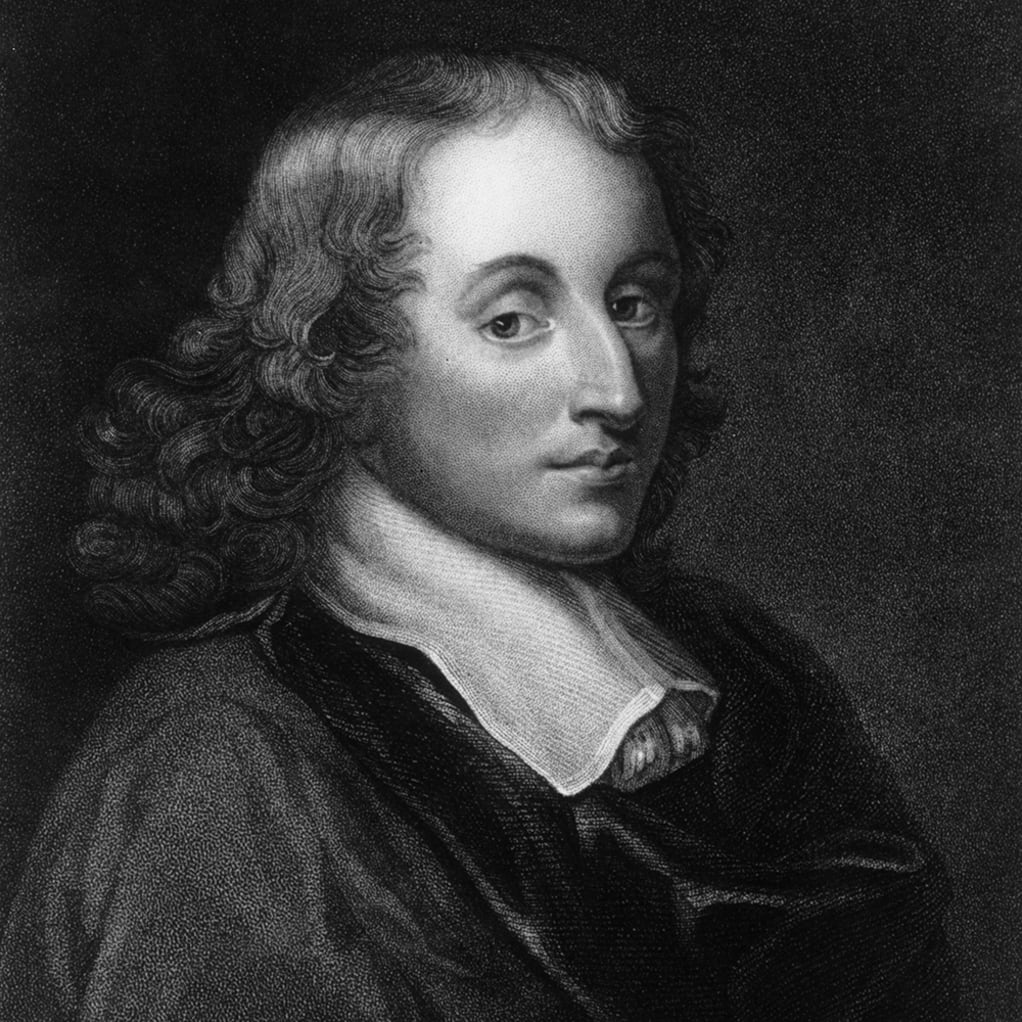
\includegraphics[width=\linewidth]{Images/ApendiceA/PASCAL.jpeg}
\textbf{\fontencoding{T1}\fontfamily{phv}\selectfont\color{cw0}Blaise Pascal:} Nacido el 19 de junio de 1623 en Clermont-Ferrand, Francia; fue un genio precoz y de clara inteligencia, pues su entusiasmo juvenil por la ciencia se materializó en importantes y precursoras aportaciones a la física y a las matemáticas. Siendo aún niño, con solo doce años, sin ayuda alguna demostró que la suma de los ángulos de un triángulo es siempre igual a 180°. Pese a su frágil salud y corta vida, murió a los treinta y nueve años, pero su huella quedó grabada en la historia de la física y de la informática.
}
\sideFigure[\label{fig:INDUCCION}Representación del Principio de Inducción]{
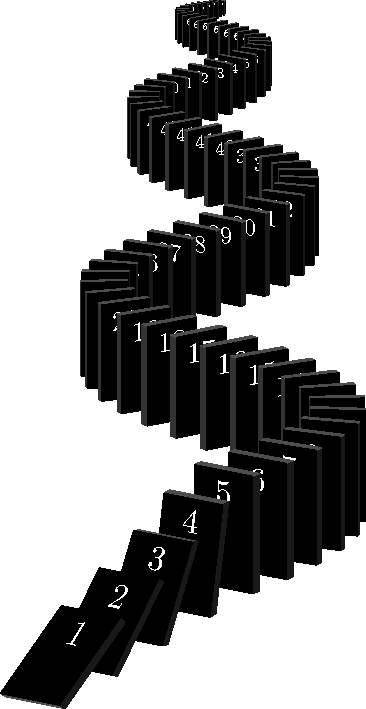
\includegraphics[width=\linewidth]{Images/ApendiceA/uuu.pdf}
}

\begin{enumerate}
    \item Todos los ciudadanos de México tienen derecho a la educación.
    \item Todos los números que terminan en cero son divisibles entre 5.
\end{enumerate}
Algunos ejemplos de proposiciones particulares son:
\begin{enumerate}
    \item Guinevere tiene derecho a la educación 
    \item 300 es divisible entre 5.
\end{enumerate}
El proceso de obtener una proposición particular de una general se llama \textbf{deducción}. Por ejemplo, si tenemos
\begin{enumerate}
    \item Todos los ciudadanos de México tienen derecho a la educación.
    \item Guinevere es mexicana.
    \item Guinevere tiene derecho a la educación.
\end{enumerate}
entonces de la proposición general (1), junto con la proposición particular (2), se obtiene la proposición particular (3).

El proceso de obtener proposiciones generales de proposiciones particulares se llama \textbf{inducción}. El razonamiento inductivo puede conducir a conclusiones falsas así como a verdaderas. Por ejemplo, si tenemos
\begin{enumerate}
    \item 300 es divisible entre 5.
    \item Todos los números que terminan en cero son divisibles entre 5.
\end{enumerate}
entonces la proposición general (2), obtenida de la proposición particular (1), es verdadera. Pero, si consideramos
\begin{enumerate}
    \item 300 es divisible entre 5.
    \item Todos los números con tres cifras son divisibles entre 5.
\end{enumerate}
entonces la proposición general (2), deducida de la proposición particular (1), es falsa.

\section{Inducción errónea en las matemáticas}

\section{El principio de la inducción matemática}

\section{El principio de buen orden}

\section{Más ejemplos de inducción}

\section{Ejercicios}

\chapter[INTRODUCCIÓN A LA PROGRAMACIÓN]{INTRODUCCIÓN A LA \\ PROGRAMACIÓN}
\printchaptertableofcontents

El lenguaje C facilita un método estructurado y disciplinado para el diseño de programas. En este apéndice introducimos la programación en C y presentamos varios ejemplos que ilustran muchas características importantes de C. Analizamos cuidadosamente cada ejemplo, línea por línea. En la sección B.7 presentamos una introducción a la programación estructurada en C. 

\section{Un programa sencillo en C: La impresión de una línea de texto}

C utiliza una notación que puede parecer extraña para quien no es programador. Comencemos considerando un programa sencillo en C. Nuestro primer ejemplo imprime una línea de texto. El programa y su resultado en pantalla aparecen en el programa \ref{Programa1}.

Aun cuando este programa es sencillo, ilustra muchas características importantes del lenguaje C. Ahora consideremos con detalle cada línea del programa. Las líneas 1 y 2:
\begin{minted}[escapeinside=]{c}
    /* Primer programa en C:
           primer_programa.c */
\end{minted}
comienzan con \mintinline{tex}{/*} y terminan con \mintinline{tex}{*/}, lo que indica que estas dos líneas son un comentario. Los programadores insertan comentarios para documentar los programas y para mejorar su legibilidad. Los comentarios no provocan que la computadora realice acción alguna durante la ejecución del programa. El compilador de C ignora los comentarios y no genera código objeto en lenguaje máquina. El comentario anterior sólo describe el número de la figura, el nombre del archivo y el propósito del programa. Los comentarios también ayudan a otras personas a leer y entender un programa, pero demasiados comentarios pueden ocasionar que un programa sea difícil de leer.

\begin{listing}[h!]
\begin{minted}[escapeinside=]{c}
    /* Primer programa en C:
           primer_programa.c */
    #include <stdio.h>
    
    /* la función main inicia la ejecución del programa */
    int main(void)
    {
        printf("Bienvenido a C!\n");
        return 0; /* indica que el programa terminó con éxito */
    } /* fin de la función main */
\end{minted}
\begin{compilado}
    Bienvenido a C!
\end{compilado}
\caption{Programa de impresión de texto}\label{Programa1}
\end{listing}
\noindent La línea 3
\begin{minted}[firstnumber=3,escapeinside=]{c}
    #include <stdio.h>
\end{minted}
\noindent es una directiva del preprocesador de C. Las líneas que comienzan con \mintinline{tex}{#} son procesadas por el preprocesador antes de que el programa se compile. Esta línea en particular indica al preprocesador que incluya en el programa el contenido del \emph{encabezado estándar de entrada/salida} (\textbf{stdio.h}). Este encabezado contiene información que el compilador utiliza cuando compila las llamadas a las funciones de la biblioteca estándar de entrada/salida, como \mintinline{c}{printf}.

La línea 6
\begin{minted}[firstnumber=6,escapeinside=]{c}
    int main(  )
\end{minted}
\noindent forma parte de todos los programas en C. Los paréntesis que aparecen después de \mintinline{tex}{main} indican que \mintinline{tex}{main} es un bloque de construcción de programas llamado función. Los programas en C contienen una o más funciones, una de las cuales debe ser \mintinline{tex}{main}. Todo programa en C comienza su ejecución en la función \mintinline{tex}{main}.

La llave izquierda (línea 7), \verb|{|, debe iniciar el cuerpo de cada función. Una llave derecha correspondiente (línea 10), debe finalizar cada función. Este par de \emph{llaves} y la parte del programa entre ellas se conocen como bloque. El bloque es una unidad importante del programa en C.

La línea 8
\begin{minted}[firstnumber=8,escapeinside=]{c}
    printf("Bienvenido a C!\n");
\end{minted}
\noindent indica a la computadora que realice una acción, es decir, que imprima en la pantalla la cadena de caracteres contenida entre las comillas. En algunas ocasiones a una cadena se le llama cadena de caracteres, mensaje o literal. La línea completa [que incluye \mintinline{c}{printf}, su argumento entre paréntesis, y el punto y coma (\verb|;|)] se conoce como instrucción. Toda instrucción debe finalizar con un punto y coma (también conocido como terminador de la instrucción). Cuando la instrucción \mintinline{c}{printf} anterior se ejecuta, esta imprime en la pantalla el mensaje \mintinline{c}{Bienvenido a C!} En general, los caracteres se imprimen exactamente como aparecen entre las comillas de la instrucción \mintinline{c}{printf}. Observe que los caracteres \mintinline{python}{\n} no aparecieron en pantalla. La diagonal invertida (\verb|\|) se conoce como carácter de escape. Este indica que se espera que \mintinline{c}{printf} haga algo fuera de lo ordinario. Cuando una diagonal invertida se encuentra dentro de una cadena, el compilador ve el siguiente carácter y lo combina con la diagonal invertida para formar una secuencia de escape. La secuencia de escape \mintinline{python}{\n} significa nueva línea. Cuando una nueva línea aparece en la salida de la cadena por medio de \mintinline{c}{printf}, esta nueva línea ocasiona que el cursor se posicione al comienzo de la siguiente línea de la pantalla. En la tabla siguiente, aparecen algunas secuencias de escape comunes.
\begin{nscenter}
    \begin{NiceTabular}{cc}[hvlines-except-borders, cell-space-limits=4pt, rules={color=white,width=1pt}]
    \CodeBefore
    \rowcolor{cw0!80}{1}
    \rowcolors{2}{cw2!70!white}{cw1!30!white}
    \Body
    \RowStyle[color=white]{}
        \RowStyle{\bfseries}\makecell{Secuencia \\ de escape} & Descripción \\
        \verb|\n| & \makecell{Nueva línea: Coloca el cursor al \\ principio de la siguiente línea} \\
        \verb|\t| & \makecell{Tabulador horizontal: Mueve el cursor \\ a la siguiente posición del tabulador} \\
        \verb|\a| & Alerta: Suena la campana del sistema \\
        \verb|\\| & \makecell{Diagonal invertida: Inserta una \\ diagonal invertida en una cadena} \\
        \verb|\"| & \makecell{Comillas: Inserta unas comillas \\ en una cadena de caracteres}
    \end{NiceTabular}
    \captionof{table}{Algunas secuencias comunes de escape}\label{tab:secuencias_de_escape}
\end{nscenter}

Las dos últimas secuencias de escape de la tabla \ref{tab:secuencias_de_escape} pueden parecer extrañas. Debido a que la diagonal invertida tiene un significado especial en una cadena, es decir, que el compilador la reconoce como un carácter de escape, nosotros utilizamos dos diagonales invertidas para colocar una sola diagonal invertida en una cadena. Imprimir comillas también representa un problema, ya que dichas comillas marcan el límite de una cadena; de hecho, estas comillas no se imprimen. Al utilizar la secuencia de escape \mintinline{matlab}{\"} en una cadena para que sea la salida de \mintinline{tex}{printf}, indicamos que \mintinline{tex}{printf} debe desplegar unas comillas.

La línea 9
\begin{minted}[firstnumber=9,escapeinside=]{c}
    return 0;
\end{minted}
\noindent se incluye al final de toda función \mintinline{c}{main}. La palabra reservada \mintinline{c}{return} representa a uno de los diversos medios que utilizaremos para salir de una función. Cuando se utiliza la instrucción \mintinline{c}{return} al final de \mintinline{c}{main}, como mostramos en este caso, el valor \mintinline{c}{0} indica que el programa finalizó exitosamente. La llave derecha (línea 10), \verb|}| indica el final de la función \mintinline{c}{main}.

Resulta importante observar que las funciones de la biblioteca estándar como \mintinline{c}{printf} y \mintinline{c}{scanf} no forman parte del lenguaje de programación C. Por ejemplo, el compilador no puede encontrar errores de escritura en \mintinline{c}{printf} o \mintinline{c}{scanf}. Cuando el compilador compila una instrucción \mintinline{c}{printf}, este sólo proporciona espacio en el programa objeto para una “llamada” a la función de biblioteca. Sin embargo, el compilador no sabe en dónde están las funciones de biblioteca; el enlazador sí lo sabe. Cuando se ejecuta el enlazador, este localiza las funciones de biblioteca e inserta las llamadas apropiadas para dichas funciones en el programa objeto. Ahora el programa objeto está “completo” y listo para ejecutarse. De hecho, al programa enlazado con frecuencia se le conoce como ejecutable. Si el nombre de la función está mal escrito, es el enlazador quien detectará el error, ya que no será capaz de hacer coincidir el nombre que se encuentra en el programa en C, con el nombre de ninguna función conocida de las bibliotecas. La función \mintinline{c}{printf} puede imprimir de diferentes formas el mensaje \mintinline{tex}{Bienvenido a C!} Por ejemplo, el programa \ref{Programa2} produce la misma salida que el programa \ref{Programa1}. 

\begin{listing}[h!]
\begin{minted}[escapeinside=]{c}
    /* Impresión de una línea mediante
           dos instrucciones printf */
    #include <stdio.h>
    
    /* la función main inicia la ejecución del programa */
    int main(void)
    {
        printf("Bienvenido ");
        printf("a C!\n");
        return 0; /* indica que el programa terminó con éxito */
    } /* fin de la función main */
\end{minted}
\begin{compilado}
    Bienvenido a C!
\end{compilado}
\caption{Programa de impresión de texto}\label{Programa2}
\end{listing}
\noindent Esto funciona porque cada \mintinline{c}{printf} continúa con la impresión a partir de donde la función \mintinline{c}{printf} anterior dejó de imprimir. La primera \mintinline{c}{printf} (línea 8) imprime \mintinline{tex}{Bienvenido} seguido por un espacio, y la segunda \mintinline{c}{printf} (línea 9) comienza a imprimir en la misma línea, inmediatamente después del espacio.
Una sola \mintinline{c}{printf} puede imprimir varias líneas utilizando caracteres de nueva línea, como en el programa \ref{Programa3}. Cada vez que aparece la secuencia de escape \mintinline{python}{\n} (nueva línea), la salida continúa al principio de la siguiente línea.
\begin{listing}[h!]
\begin{minted}[escapeinside=]{c}
    /* Impresión de múltiples líneas mediante
           una sola instrucción printf */
    #include <stdio.h>
    
    /* la función main inicia la ejecución del programa */
    int main(void)
    {
        printf("Bienvenido\na\nC!\n");
        return 0; /* indica que el programa terminó con éxito */
    } /* fin de la función main */
\end{minted}
\begin{compilado}
    Bienvenido\\
    a\\
    C!
\end{compilado}
\caption{Programa de impresión de texto}\label{Programa3}
\end{listing}

\section{Otro programa sencillo en C: La suma de dos números enteros}

Nuestro siguiente programa utiliza la función \mintinline{c}{scanf} de la biblioteca estándar para obtener dos enteros escritos por el usuario a través del teclado, para calcular la suma de dichos valores e imprimir el resultado mediante \mintinline{c}{printf}. El programa y el resultado del ejemplo aparecen en el programa \ref{Programa4}. Observe que en el diálogo de entrada/salida del programa \ref{Programa4} resaltamos los números introducidos por el usuario.
\begin{listing}[h!]
\begin{minted}[escapeinside=]{c}
    /* Programa para poder
           sumar dos números enteros */
    #include <stdio.h>
    
    /* la función main inicia la ejecución del programa */
    int main()
    {
        int entero1; /* primer número a introducir por el usuario */
        int entero2; /* segundo número introducir por el usuario */
        int suma; /* variable en la que se almacenará la suma */

        printf("Introduzca el primer entero\n"); /* indicador */
        scanf("%d", &entero1); /* lee un entero */

        printf("Introduzca el segundo entero\n"); /* indicador */
        scanf("%d", &entero2); /* lee un entero */

        suma = entero1 + entero2; /* asigna el resultado a suma */

        printf("La suma es %d\n", suma); /* imprime la suma */
        
        return 0; /* indica que el programa terminó con éxito */
    } /* fin de la función main */
\end{minted}
\begin{compilado}
    Bienvenido a C!
\end{compilado}
\caption{Programa de impresión de texto}\label{Programa4}
\end{listing}

\end{document}
